\documentclass[magister,druk]{dyplom}
\usepackage[utf8]{inputenc}

\usepackage{graphicx}
\usepackage{wrapfig}
\usepackage{float}
\usepackage{multirow}

\graphicspath{{C:/Users/Kateryna/Documents/thesis/pictures/}}

\author{Kateryna Dlugunovych}
\title{Badania wytrzymałościowe połączenia stopu aluminium z kompozytem na osnowie PE}
\titlen{Testing the strength of the connection of the aluminium with PE matrix composite}
\promotor{dr Oliwia Trzaska}
\konsultant{dr Wojciech Błażejewski}
\wydzial{Wydział Mechaniczny}
\kierunek{Mechanika i Budowa Maszyn}
\specjalnosc{Inżynieria Materiałów Konstrukcyjnych}

\begin{document}	

\maketitle

\tableofcontents

\chapter{Wstęp teoretyczny}
\section{Streszczenie}
\section{Cel i zakres pracy}
Celem pracy jest zbadanie możliwości połączenia stopu aluminium z materiałem na osnowie PE.

Zakres pracy obejmuje zbudowanie stanowiska, przygotowanie próbek, przeprowadzenie badań wytrzymałościowych oraz analizę wyników.
\section{Klasyfikacja materiałów kompozytowych}

Kompozyt zgodnie z definicją to materiał, składający się z dwóch lub więcej składników o różniących się właściwościach fizycznych lub chemicznych, które po połączeniu stwarzają materiał o właściwościach odmiennych od podstawowych składników. 

Materiały kompozytowe mogą być używane ze względu na niekonwencjonalne kombinacje wytrzymałości, sztywności, ciężaru właściwego, własności w podwyższonych temperaturach, odporności na korozję, twardości lub przewodności.

Uogólniając powyższe, materiały kompozytowe składają się z dwóch faz: ciągłej, nadającej kształt i wygląd, oraz rozproszonej, wnoszącej określone właściwości kompozytu.

Ze względu na typ matrycy(fazy ciągłej), można podzielić kompozyty na trzy rodzaje:
\begin{itemize}	
\item metalowe
\item ceramiczne
\item polimerowe
\end{itemize}

Najczęściej kompozyty o osnowie metalowej (MMC) występują z wzmocnieniem ceramicznym (cermetale), ale mogą również być wzmacniane metalami lub stopami odmiennymi od osnowy, jak i zwykłymi włóknami (szklane, węglowe, aramidowe, i t.p.). MMC są często stosowane w branży motoryzacyjnej oraz lotniczej ze względu na ulepszone właściwości mechaniczne podczas pracy w wysokich temperaturach\cite{MMC}. Przykładem może być wykorzystanie aluminium częściowo wzmocnionego włóknami $Al_{2}O_{3}$. Porównywalne właściwości danego węzła konstrukcyjnego można uzyskać używając tłoków zrobionych z żelaza(podwyższona masa) lub sproszkowanego aluminium powder metallurgical aluminum alloys (droga technologia).

Kompozyty o osnowie ceramicznej znacząco się różnią od konwencjonalnych materiałów kompozytowych. Materiały ceramiczne charakteryzują się wysoką twardością, odpornością na wysoką temperaturę, korozję oraz oddziaływania chemiczne. Zazwyczaj w kompozytach większe obciążenie powinno przenosić włókno wzmacniające. W przypadku kompozytów o osnowie ceramicznej wzmocnienie powinno pomóc zachować odporność na wysokie temperatury i wpływ otoczenia, oraz zapewnić wytrzymałość materiału(skompensować wysoką kruchość ceramiki).
     
\begin{figure}[H]
	\begin{center}
		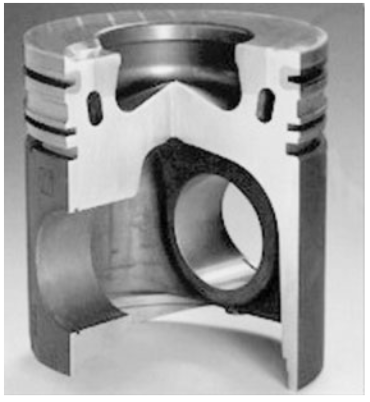
\includegraphics[width=0.5\textwidth]{MMCpiston}
		%\rule{3cm}{7cm}
		\centering
	\end{center}
	\caption{Tłok z wykorzystaniem MMC//Partial short fiber reinforced
				light metal diesel pistons  }
\end{figure}

 

Kompozyty o osnowie polimerowej zostaną dokładnie opisane w następnym podrozdziale.

Ze względu na strukturę wzmocnienia(fazy rozproszonej), rozróżnia się dwa podstawowe rodzaje kompozytów:
\begin{itemize}
\item kompozyty włókniste
\item kompozyty cząstkowe, ziarniste, proszkowe
\end{itemize}

Wzmocnienie jest uważane za włókniste, gdy wymiary wzdłużne cząstek są znacznie większe od wymiarów poprzecznych. W przypadku wzmocnienia cząstkowego wszystkie trzy wymiary cząstki są zbliżonej wielkości.

Istotnym czynnikiem wpływającym na właściwości wytrzymałościowe kompozytów jest kształt cząstek fazy rozproszonej, a w przypadku cząstek włóknistych ich współczynnik kształtu (stosunek długości do średnicy). Im on jest większy tym lepsze są właściwości mechaniczne kompozytu (lepsze przenoszenie naprężeń z fazy wiążącej na włókna).\cite{Krolikowski2012}

\begin{figure}
	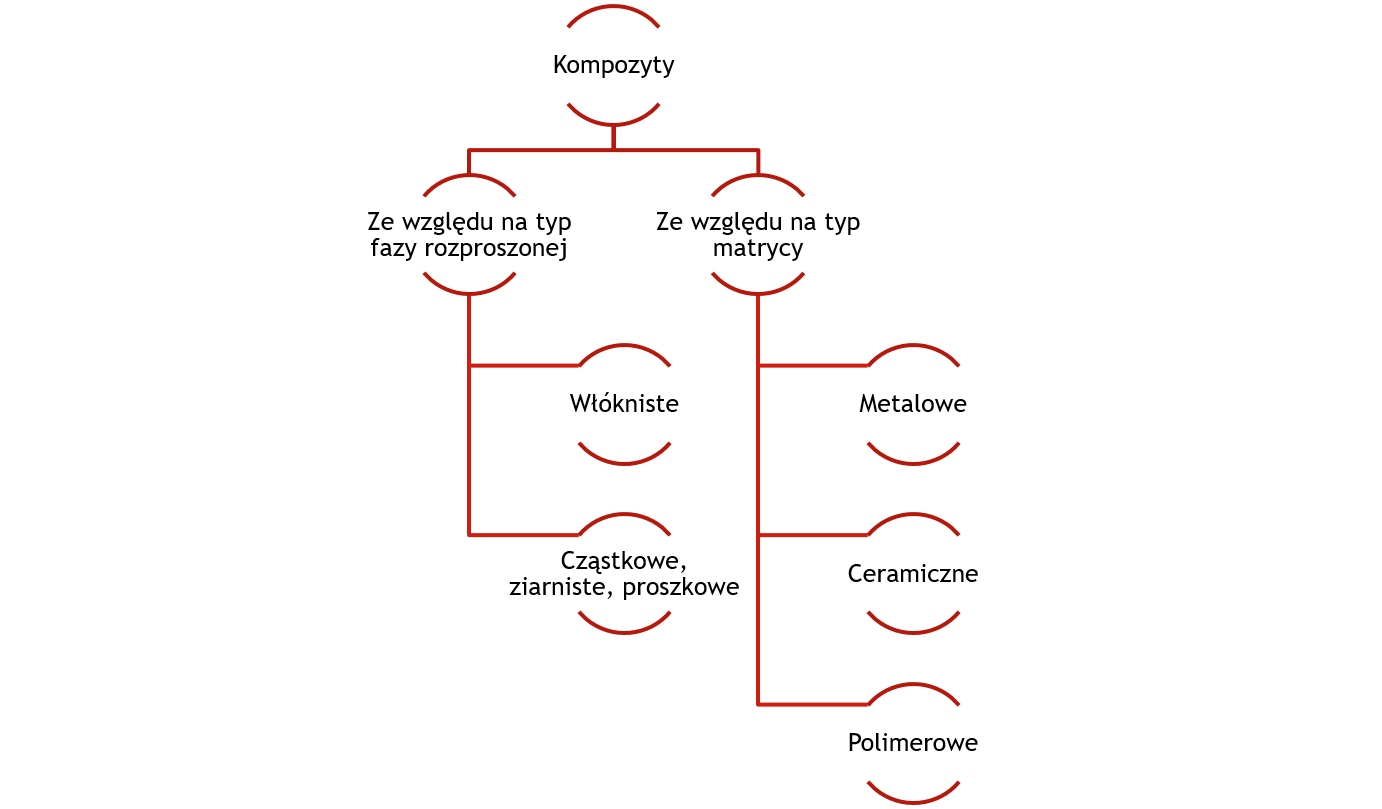
\includegraphics[width=1\textwidth]{Classification}
	\caption{Klasyfikacja materiałów kompozytowych}
\end{figure}


\section{Polimerowe kompozyty wzmacniane włóknami}
 
Z punktu widzenia właściwości oraz obszaru zastosowań można podzielić kompozyty polimerowe na dwie grupy:
\begin{itemize}
	\item kompozyty funkcjonalne
	\item kompozyty konstrukcyjne
\end{itemize}

Kompozyty funkcjonalne posiadają specyficzne właściwości, które powodują że takie materiały mają wąski, ściśle określony obszar zastosowań. Przykładem mogą być kompozyty elektryczne, magnetyczne, optyczne, ślizgowe, przeciwogniowe, barierowe, itp \cite{Krolikowski2012}.
 
Kompozyty konstrukcyjne są materiałami o dobrych właściwościach mechanicznych oraz małym ciężarze właściwym. Dzięki opisanym wyżej właściwościom są szeroko stosowane w elementach konstrukcyjnych maszyn, konstrukcjach budowlanych oraz przedmiotach codziennego użytku.

Składnikami polimerowych kompozytów konstrukcyjnych są:
\begin{itemize}
	\item polimery stanowiące fazę ciągłą
	\item faza rozproszona (cząsteczki, włókna)
	\item dodatki uzupełniające
	\item materiały dodatkowe do konstrukcji przekładkowych
\end{itemize} 
 
\subsection{Osnowy polimerowe materiałów kompozytowych, osnowy termoplastyczne}

Szerokie zastosowanie jako osnowy konstrukcyjnych materiałów kompozytowych mają polimery termoutwardzalne, takie jak nienasycone żywice poliestrowe i winyloestrowe, a także fenolowo-formaldehydowe żywice rezolowe, poliimidy, silikony oraz sieciowane poliuretany\cite{Krolikowski2012}.

Żywica poliestrowa stosowana jako osnowa w kompozytach jest roztworem oligoestru nienasyconego w styrenie (ok. 30-40 \%). Utwardzanie żywic poliestrowych odbywa się poprzez kopolimeryzację oligoestru z styrenem przy udziale podwójnych wiązań obu składników. Cząsteczki styrenu wbudowują się pomiędzy łańcuchy oligoestru, wskutek tego powstaje sieć przestrzenna. Od gęstości sieci zależą właściwości mechaniczne uzyskanego materiału (moduł E, twardość, wydłużenie przy zerwaniu, ugięcie cieplne). Kopolimeryzacja odbywa się pod wpływem inicjatorów  wolnorodnikowych (utwardzaczy). Dane związki, pod wpływem wysokiej temperatury lub przyspieszaczy, rozpadając tworzą wolne rodniki, umożliwiające kopolimeryzację.

W procesie wytwarzania kompozytów z żywic poliestrowych używane są dwa sposoby utwardzenia: na gorąco (ok. $160 C^{\circ}$) i na zimno (w temperaturze pokojowej, powyżej $15 C^{\circ}$). Przy utwardzaniu na gorąco stosuje się odpowiednie prasy z ogrzewanymi formami z dedykowanym inicjatorem nadtlenkowym (np. nadbenzoesan III-rzędowego butylu). W formowaniu wyrobów kompozytowych na zimno stosuje się zespół utwardzaczy - inicjator wodoronadtlenkowy z przyspieszaczem (sole kobaltu lub inne aminy), umożliwiającym utwardzanie wyrobu w temperaturze pokojowej. Dużą zaletą żywic poliestrowych jest łatwość w stosowaniu, niska cena, łatwa przesycalność włókien oraz uniwersalność. Wadami są właściwości mechaniczne, duża emisja styrenu, palność, skurcz przy utwardzaniu oraz mała odporność korozyjna.

Żywice winyloestrowe charakteryzują się strukturą chemiczną, u której w oligomerycznym łańcuchu znajduje się fragment żywicy epoksydowej, a na końcach są umieszczone grupy estrowe i grupy winylowe zawierające wiązania podwójne. Dane żywice mają lepsze właściwości mechaniczne, cieplne i większą odporność chemiczną niż żywice poliestrowe. Z drugiej strony, cechują się dużą zawartością styrenu, bardzo dużym skurczem przy utwardzaniu oraz wyższą ceną. 

Żywice epoksydowe mają zróżnicowaną budowę chemiczną, ale do zastosowań kompozytowych używane są żywice bisfenolowe o różnym ciężarze cząsteczkowym. Liczba hydroksylowa opisuję zawartość grup hydroksylowych, wraz z jej wzrostem rośnie ciężar cząsteczkowy, lepkość i temperatura mięknięcia, liczba epoksydowa wówczas maleje. Utwardzanie kompozytów na podstawie żywic epoksydowych w temperaturze pokojowej odbywa się za pomocą utwardzaczy w postaci amin pierwszorzędowych różnego rodzaju. W temperaturach powyżej $100 C^{\circ}$ stosowane są związki typu kwasów Lewisa lub amin typu aromatycznego. Zaletami danych żywic są bardzo dobre właściwości mechaniczne, termiczne i antykorozyjne, mały skurcz przy utwardzaniu i dobra adhezja do włókien wzmacniających. Wady to wysoka cena, duża lepkość, toksyczne utwardzacze oraz dodatkowe koszty stosowania modyfikatorów. 

\begin{table}[H]
	\centering
	\caption{Właściwości utwardzonych żywic}
	\label{my-label}
	\resizebox{\textwidth}{!}{
	\begin{tabular}{|l|c|c|c|}
		\hline
		\multicolumn{1}{|c|}{\multirow{2}{*}{Właściwości}} & \multicolumn{3}{c|}{Żywice}              \\ \cline{2-4} 
		\multicolumn{1}{|c|}{}                             & poliestrowe & winyloestrowe & epoksydowe \\ \hline
		Gęstość, {[}$ \frac{g}{cm^{3}} $ {]}                                & 1,23        & 1,04          & 1,14       \\ \hline
		Wytrzymałość na rozciąganie, {[}MPa{]}              & 70          & 85            & 75         \\ \hline
		Moduł sprężystości E, {[}GPa{]}                     & 3,8         & 3,3           & 3          \\ \hline
		Wydłużenie przy zerwaniu $\varepsilon_{m}$, {[}\%{]}                    & 2,3         & 5             & 5          \\ \hline
		Współczynnik rozszerzalności cieplnej,{[} $ \frac{10^{-6}}{C^{\circ}} $ {]}     & 160-80      & 60            & 120-80     \\ \hline
	\end{tabular}
	}
\end{table}

Polimery termoplastyczne stosowane w materiałach kompozytowych to poliolefiny, poliamidy, polichlorek winylu, poliwęglany, termopolimery ABS oraz poliestry nasycone (PET, PBT)\cite{Krolikowski2012}. 

Najważniejsze poliolefiny w przemyśle kompozytowym to polietylen i polipropylen. Polietylen jest pochodną etylenu otrzymywaną za pomocą polimeryzacji metodą wysoko- lub niskociśnieniową. Metodą wysokociśnieniową otrzymuje się polietylen o niskiej gęstości - LDPE (Low Density Polyethylene), posiadający silnie rozgałęziony łańcuch (8-40 rozgałęzionych łańcuchów na 1000 członów łańcucha podstawowego). Za pomocą metody niskociśnieniowej wytwarza się polietylen o wysokiej gęstości - HDPE (High Density Polyethylene), z mało rozgałęzionym łańcuchem (ok. 5 łańcuchów bocznych na 1000 członów). 

\begin{figure}[H]
	\centering
	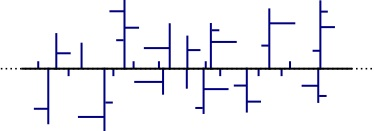
\includegraphics[width=0.5\textwidth]{LDPE}
	\caption{Schemat struktury LDPE\cite{wiki}}
\end{figure}

\begin{figure}[H]
	\centering
	\includegraphics[width=0.5\textwidth]{HDPE}
	\caption{Schemat struktury HDPE\cite{wiki}}
\end{figure}

Nazwą poliamidy określa się częściowo krystaliczne łańcuchowe termoplasty. Metoda wytwarzania to polikondensacja kwasów dikarboksylowych oraz amin, lub polimeryzacja laktamów kwasów aminokarboksylowych. Poliamidy PA6 i PA66 stosowane są w postaci kompozytowych granulatów wzmocnionych włóknem szklanym. Temperatury wtrysku wynoszą od 230 do 320 ${C^{\circ}}$, skurcz formowniczy wynosi ok. 2 \% objętości.

\begin{figure}[H]
	\centering
	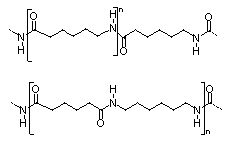
\includegraphics[width=0.5\textwidth]{PA6}
	\caption{Schemat struktury PA6(powyżej) i PA66(poniżej)\cite{wikiPA}}
\end{figure}

Poliestry termoplastyczne - PET(politereftalan etylenu) i PBT(politereftalan butylenu) - w odróżnieniu od poliestrów nienasyconych, będących oligomerami, są nasyconymi łańcuchowymi wielkocząsteczkowymi polimerami termoplastycznymi. Stopień krystaliczności wyrobów z PET i PBT jest regulowany za pomocą parametrów termicznych przetwórstwa. Z danych materiałów wytwarzane są granulaty wzmocnione szklanym włóknem ciętym oraz płyty z tkaninami, matami lub włókninami szklanymi.

% Please add the following required packages to your document preamble:
% \usepackage{multirow}
% \usepackage{graphicx}
\begin{table}[H]
	\centering
	\caption{Orientacyjne właściwości polimerów termoplastycznych}
	\label{my-label}
	\resizebox{\textwidth}{!}{%
		\begin{tabular}{|l|c|c|c|c|c|c|}
			\hline
			\multicolumn{1}{|c|}{\multirow{2}{*}{Właściwości}}                      & \multicolumn{2}{c|}{Polietyleny} & \multicolumn{2}{c|}{Poliamidy} & \multicolumn{2}{c|}{Poliestry termoplastyczne} \\ \cline{2-7} 
			\multicolumn{1}{|c|}{}                                                  & LDPE             & HDPE          & PA6           & PA66           & PET                    & PBT                   \\ \hline
			Gęstość {[}g/cm3{]}                                                     & 0,915-0,920      & 0,94-0,96     & 1,12          & 1,13-1,16      & 1,33-1,40              & 1,30-1,32             \\ \hline
			Moduł E przy rozciąganiu {[}MPa{]}                                      & 200-400          & 600-1400      & 1200          & 1500           & -                      & -                     \\ \hline
			Wytrzymałość na rozciąganie {[}MPa{]}                                   & -                & -             & 64            & 63             & -                      & -                     \\ \hline
			Naprężenie na granicy plastyczności {[}MPa{]}                           & 8-10             & 18-30         & -             & -              & 55-80                  & 50-60                 \\ \hline
			Temperatura topnienia {[}$C^{\circ}${]}                                 & 105-118          & 126-135       & 220-225       & 225-260        & 250-260                & 220-225               \\ \hline
			Współczynnik rozszerzalności liniowej {[}$\frac{10^{-3}}{C^{\circ}}${]} & 160-80           & 60            & -             & -              & -                      & -                     \\ \hline
			Temperatura ugięcia HDT/A cieplnego 1,8 MPa, ${C^{\circ}}$              & 30-37            & 38-50         & 80            & 66-85          & 60-75                  & 50-65                 \\ \hline
		\end{tabular}%
	}
\end{table}

\subsection{Wzmocnienia materiałów kompozytowych}

Wzmocnienia materiałów kompozytowych zmieniają właściwości fizyczne osnowy, hamują propagację pęknięć, nadają specyficzne właściwości(ślizgowe, przewodzące, antyelektrostatyczne, zmniejszające palność, itp.), oraz wpływają na wygląd wyrobu. Ze względu na kształt fazy rozproszonej wyróżnia się napełniacze ziarniste, whiskery, krótkie włókna, długie włókna oraz tkaniny. 

Napełniacze ziarniste mogą być mieć różne pochodzenie: naturalne, syntetyczne, mineralne lub organiczne. Często stosowane napełniacze to różne rodzaje sadz, grafit, proszki i płatki metali. Właściwości układów kompozytów polimerowych z napełniaczami zależą od ich ilości, właściwości, stopnia rozdrobnienia, wzajemnej adhezji oraz zwilżalności. 

Najczęściej używane w kompozytach są wzmocnienia w formie włóknistej ze względu na 
następujące czynniki\cite{Dresher}:
\begin{itemize}
	\item Mała średnica w stosunku do jednostki mikrostrukturalnej. Ze względu na efekt rozmiaru (z ang. size effect), prawdopodobieństwo wystąpienia niedoskonałości jest mniejsze w materiale o mniejszych wymiarach, więc zakłada się że ma wyższą wytrzymałość.
	\item Wysoki współczynnik kształtu (stosunek długości włókna do jego średnicy - $\frac{l}{d}$), który umożliwia transfer dużej części obciążenia przez osnowę do wytrzymałego włókna.
	\item Duża podatność (elastyczność). Dla włókna (długa cienka belka), podatność jest odwrotnie proporcjonalna do sztywność oraz średnicy\cite{Chawla1998}. Dzięki temu, dla odpowiednio małych średnic można uzyskać elastyczne włókna z kruchych materiałów, takich jak szkło, węgiel, kwarc, itp.    
\end{itemize}

\begin{figure}[H]
	\centering
	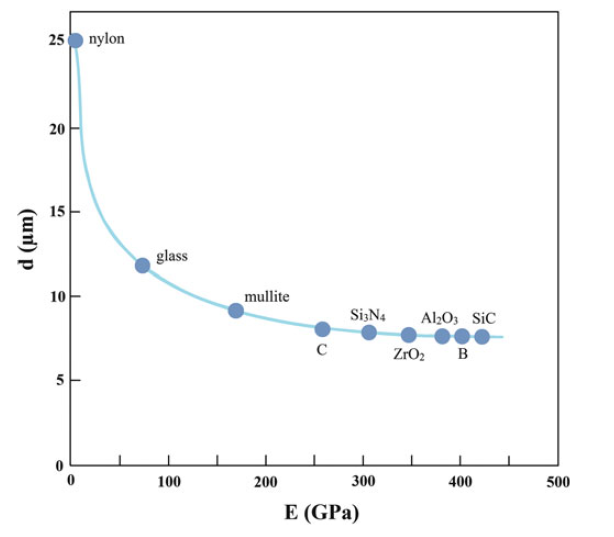
\includegraphics[width=0.8\textwidth]{diameter}
	\caption{Średnicy włókien różnych materiałów o podatności włókna PA66 o średnicy 25 $\mu m$)\cite{Chawla1998}}
\end{figure}

Ze względu na materiał używane są następujące rodzaje włókien:
\begin{itemize}
	\item szklane
	\item aramidowe
	\item bazaltowe
	\item kwarcowe
	\item węglowe i grafitowe
	\item polimerowe
	\item inne
\end{itemize}

Włókna szklane to nazwa ogólna włókien na bazie tlenku krzemu (50-60\%), zawierających także tlenki wapnia, boru, sodu, glinu, itp. Są podstawowym, powszechnie stosowanym wzmocnieniem szerokiej gamy polimerów. Technologia wytwarzania oraz metody przetwarzania są w pełni opracowane, co skutkuje dobrą jakością oraz niską ceną. W kompozytach o osnowie polimerowej głównie są stosowane włókna ze szkła boro-glino-krzemowego, oznaczane symbolem E (elektroizolacyjne). Pomimo szerokiej gamy zastosowań nie są uznawane za optymalne, gdyż posiadają małą wytrzymałość mechaniczną, mały moduł sprężystości oraz są podatne na korozję. Właściwości włókien szklanych zależą od zawartości tlenków więźbotwórczych, średnicy włókien, parametrów wytwarzania oraz typu szkła.

\begin{figure}[]
	\centering
	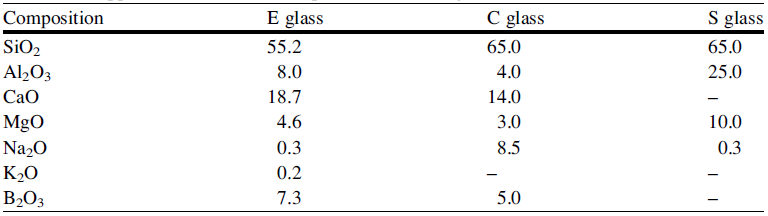
\includegraphics[width=0.8\textwidth]{glassfiber}
	\caption{Składy chemiczne wybranych włókien szklanych\cite{Chawla1998}}
\end{figure}

Włókna bazaltowe to ciemnografitowe włókna, wytwarzane ze skał wulkanicznych. Ze względu na różny skład skał, właściwości włókien różnią się w zależności od wytwórcy. Odporność termiczna (580-650 ${C^{\circ}}$) i korozyjna, wytrzymałość oraz moduł sprężystości są wyższe (10-15\% i 20-25\% odpowiednio) niż dla standardowych włókien szklanych.

W postaci rovingu, włókien ciętych, tkanin i mat są dostępne włókna kwarcowe. Ich standardowy typ odporny jest do temperatury 1050 ${C^{\circ}}$, wytrzymałość na zerwanie 6000 MPa, moduł E 78 GPa, wydłużenie 7,7\%. Właściwości danych włókien są dużo lepsze niż dla włókien szklanych, ale cena jest również dużo wyższa.

Pierwiastki węgla w odmianie grafitowej posiadają wysoko anizotropowe właściwości, ze względu na warstwową strukturę o bardzo gęste upakowaniu. Wobec tego, w procesie wytwarzania włókien węglowych dąży się do uzyskania struktury heksagonalnej w osi włókna. Początkowo wytwarzane były w procesie pirolizy z celulozy. Obecnie są wytwarzane z zastosowaniem prekursorów w postaci poliakrylonitrylu (PAN) oraz paków mezofazowych. Przechodzą one etapy oksydacji (przekształcenie w materiał usieciowany i nietopliwy), karbonizacji (piroliza bez topnienie oraz aromatyzacji struktury włókien), oraz grafityzacji. W efekcie tych procesów, uzyskuje się wartości wytrzymałości na rozciąganie do ok. 2500 MPa i modułu E ok. 400 GPa, w zależności od parametrów procesu. Struktura i właściwości włókien zależą znacznie od składu i struktury prekursora, parametrów technologicznych wytwarzania, oraz od stopnia orientacji pasm krystalitów grafitu w stosunku do osi włókna.

Aramidy - aromatyczne poliamidy, to liotropowe polimery ciekłokrystaliczne. Wytwarzane są w podstawowych typach Nomex, Kevlar oraz Twaron. Włokna Nomex posiadają znakomitą odporność cieplną i chemiczną, małą palność oraz bardzo dobre właściwości elektryczne. Kevlar posiada dużą wytrzymałość i duży moduł sprężystości. 

Włókna polietylenowe o dużej wytrzymałości na rozciąganie i dużym modułem sprężystości, są znane pod nazwą Dyneema. Do wytwarzania używa się polietylenu o szczególnie dużym ciężarze cząsteczkowym UHMWPE (ang. ultra high molecular weight polyethylene), który ma bardzo duży stopień polimeryzacji (ok. 100000, dla HDPE wynosi ok.700-1800). Technologia wytwarzania - ang. gelspinning - obejmuje przędzenie z żelu. Wyjściowy UHMWPE jest rozpuszczany w dobranym rozpuszczalniku, wskutek czego poszczególne łańcuchy są izolowane oraz rozprostowywane. Typ włókien oraz ich właściwości fizyczne i mechaniczne są regulowane poprzez dobór wyjściowego UHMWPE i zmianę parametrów przędzenia. 

% Please add the following required packages to your document preamble:
% \usepackage{multirow}
% \usepackage{graphicx}
% Please add the following required packages to your document preamble:
% \usepackage{multirow}
% \usepackage{graphicx}
\begin{table}[]
	\centering
	\caption{Porównanie właściwości włókien \cite{Krolikowski2012}}
	\label{my-label}
	\resizebox{\textwidth}{!}{%
		\begin{tabular}{|l|l|l|l|l|l|}
			\hline
			\multicolumn{1}{|c|}{\multirow{2}{*}{Właściwości}} & \multicolumn{5}{c|}{Włókna} \\ \cline{2-6} 
			\multicolumn{1}{|c|}{} & \multicolumn{1}{c|}{Kevlar 29} & \multicolumn{1}{c|}{Kevlar 49} & \multicolumn{1}{c|}{grafitowe} & \multicolumn{1}{c|}{szklane E} & \multicolumn{1}{c|}{\begin{tabular}[c]{@{}c@{}}polietylenowe \\ Dyneema\end{tabular}} \\ \hline
			Gęstość, g/cm3 & 1,44 & 1,45 & 1,75 & 2,55 & 0,97 \\ \hline
			Wytrzymałość na rozciąganie, MPa & 3620 & 3620 & 3150 & 2450 & 2600-3050 \\ \hline
			Moduł E przy rozciąganiu, GPa & 58 & 120 & 224 & 73 & 90-175 \\ \hline
			Wydłużenie przy zerwaniu, \% & 3,7 & 1,9 & 1,25 & 1,5-3,5 & 2,7-3,5 \\ \hline
		\end{tabular}%
	}
\end{table}

\subsection{Technologie wytwórcze}

Metody wytwarzania wyrobów kompozytowych z użyciem polimerów termoplastycznych są następujące:
\begin{itemize}	
	\item formowania metodą wtrysku granulatów wzmocnionych
	\item wytwarzanie płyt z termoplastów wzmocnionych matą, włókniną lub tkaniną
	\item formowanie prefabrykatów płaskich metodą próżniową lub ciśnieniową z workiem
	\item formowanie ciśnieniowe w prasach
	\item formowanie profili metodą ciągłą pultruzji
	\item formowanie metodami nawijania i AFP
	\item metody R-RIM i S-RIM
	\item formowanie wyrobów sposobem ciśnieniowym "na zimno"
\end{itemize}

Do metody formowania wtryskowego niezbędne jest odpowiednie przygotowanie granulatu - mieszanki polimeru z włóknem (najczęściej szklanym). Dla produkcji granulatu z włóknem ciętym służy dwuślimakowa wytłaczarka z segment mieszającym. Tak przygotowany granulat jest wtryskiwany do formy w wtryskarce ślimakowej. Dla uzyskania wtryskowych termoplastów z długimi włóknami, roving jest impregnowany w głowicy krzyżowej wytłaczarki lub wprowadzany bezpośrednio w strefę ślimaków wytłaczarki.

Termoplasty wzmocnione matami szklanymi są produkowane w klasycznej technologii wytłaczania. Polega to na stosowaniu dwóch cienkich folii PP, pomiędzy które umieszcza się dwie warstwy mat rovingowych ciętych lub ciągłych i w środku bezpośrednio znajduje się dość gruba, gorąca warstwa PP. Taki zespół przechodzi przez sekcje ogrzewające i chłodzące, po czym jest cięty na płyty i pakowany. 

W metodzie RIM stosuje się substraty dwufunkcyjne. Polega ona na dokładnym dozowaniu w sposób ciągły substratów, które są mieszane w głowicach udarowych. Wytworzona kompozycja jest wstrzykiwana pomiędzy dwie połowy sztywnej formy (z ułożonym włoknem wzmacniającym), gdzie powstaje kompozyt. 

Wytwarzanie profili z matrycami termoplastycznymi może być prowadzone dwoma sposobami. Pierwszym sposobem jest impregnacja włókien ciągłych ciekłymi substratami, z których w głowicy formującej w podwyższonych temperaturach zachodzą reakcje chemiczne powstawania polimeru. Bardziej powszechną metodą jest impregnacja włókien ciągłych polimerami stopionymi, lub roztworami termoplastów albo rovingów preimpregnowanych. W urządzeniu do wytwarzania profili z termoplastów, jest impregnator w którym włókna wzmacniające są impregnowane pod ciśnieniem stopu polimeru ze zbiornika ciśnieniowego, ogrzanego do temperatury topnienia lub płynięcia polimeru\cite{Krolikowski2012}. W przypadku stosowania włókien preimpregnowanych, nieobecny jest zbiornik ciśnieniowy. 

Nawijanie wyrobów z użyciem termoplastów odbywa się na metalowym obracającym się rdzeniu, gdzie kompozycja ulega schłodzeniu i zestaleniu. Wcześniej materiał wyjściowy (preimpregnaty, włókna nawijane razem z folią lub wzmocnienia z włókien mieszanych) jest podgrzewany, następnie odbywa się proces nawijania z dociskiem materiału do rdzenia. 

\begin{figure}[H]
	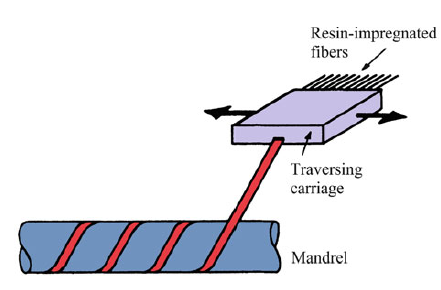
\includegraphics[width=1\textwidth]{nawijanie}
	\caption{Metoda nawijania\cite{Chawla1998}}
\end{figure}

\begin{figure}[H]
	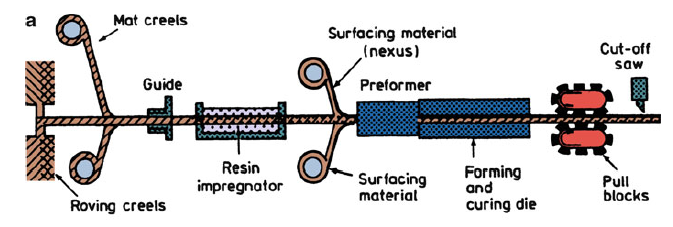
\includegraphics[width=1\textwidth]{pulltruzion}
	\caption{Metoda pultruzji\cite{Chawla1998}}
\end{figure}

\section{Zastosowanie materiałów kompozytowych}
\section{Połączenie metal kompozyt}

Laminaty metalowo-włókniste (Fiber Metal Laminates) składają się z kilku cienkich warstw metalu połączonych poprzez warstwy kompozytu. Taki materiał zachowuje się jak zwykła struktura metaliczna, ale łączy w sobie właściwości zarówno metalu, jak i materiału kompozytowego wzmacnianego włóknami. FML charakteryzują się wysoką tolerancją uszkodzeń, wysoką wytrzymałością zmęczeniową, odpornością na uderzenia, odpornością na korozję oraz ognioodpornością\cite{FML}. 

Kompozyty FML zostały opracowane na uniwersytecie technicznym w Delft na początku lat 80., najpierw pod nazwą ARALL (Aramid Reinforced Aluminium Laminates) and then GLARE (GLAss REinforced aluminium). W trakcie rozwoju materiałów o lepszej odporności na pękanie wywnioskowano, że rozrost pęknięć może być ograniczany w warstwowym, połączonym adhezyjnie materiale. Jeśli pęknięcie powstaje w jednej z warstw materiału, pozostałe ograniczają jego rozrost. Dzięki temu, pęknięcia mogą się rozwijać we wszystkich warstwach bez wzajemnej interferencji. 



\begin{figure}[H]
	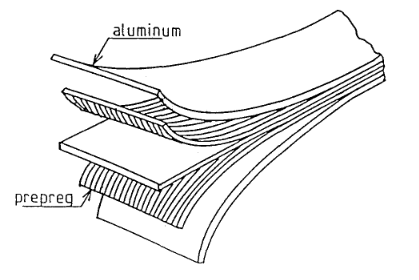
\includegraphics[width=0.5\textwidth]{FML}
	\centering
	\caption{Schemat FML\cite{FMLold}}
\end{figure}

\subsection{Wytwarzanie FML}

Najbardziej powszechną metodą wytwarzania FML jest technika autoklawowa (wysokie ciśnienie, podciśnienie, podwyższona temperatura). 

\subsection{Fizyka połączenia}

\chapter{Opracowanie konstrukcji stanowiska badawczego}
\section{Założenia konstrukcyjne}
\section{Przyjęte rozwiązania}

\chapter{Wykonanie konstrukcji stanowiska badawczego}
\section{Proces powstawania stanowiska}
\section{Próby ruchowe - podsumowanie}

\chapter{Metodyka badań}
\section{Wykonanie próbek}

Pierwsze udane próbki zostały wykonane za pomocą wycięcia w środku pręta, do którego została wsypana mieszanka proszku PE oraz ziaren korundu(ok. 15 \%). Czas docisku był uwarunkowany stanem materiału - pojawieniem się charakterystycznego ubytku(plastyczna mieszanka pyłu aluminium oraz spoiwa) świadczącego o przejściu PE do stanu płynnego. 

\section{Parametry zmienne}




\begin{table}[H]
	\centering
	\caption{Parametry zmienne w badaniach}
	\label{my-label}
	\resizebox{\textwidth}{!}{%
		\begin{tabular}{|l|l|l|l|l|l|l|}
			\hline
			\# & Czas docisku {[}min{]} & Ilość korundu {[}\%{]} & \begin{tabular}[c]{@{}l@{}}Ilość włókna\\ szklanego {[}\%{]}\end{tabular} & \begin{tabular}[c]{@{}l@{}}Głębokość\\ wycięcia {[}mm{]}\end{tabular} & \begin{tabular}[c]{@{}l@{}}Średnica\\ wewnętrzna {[}mm{]}\end{tabular} & \begin{tabular}[c]{@{}l@{}}Prędkość\\ obrotowa {[}obr/min{]}\end{tabular} \\ \hline
			1. & 1.5 & 15 & 0 & 1 & 16 & 710 \\ \hline
			2. & 2 & 15 & 0 & 2 & 18 & 710 \\ \hline
			3. & 2 & 20 & 0 & 2 & 16 & 710 \\ \hline
			4. & 3 & 20 & 0 & 2 & 18 & 710 \\ \hline
		\end{tabular}%
	}
\end{table}

\section{Badania wytrzymałościowe}
\subsection{Badania wytrzymałości na zginanie}
\subsection{Badania wytrzymałości na skręcanie, rozciąganie}

\begin{figure}
	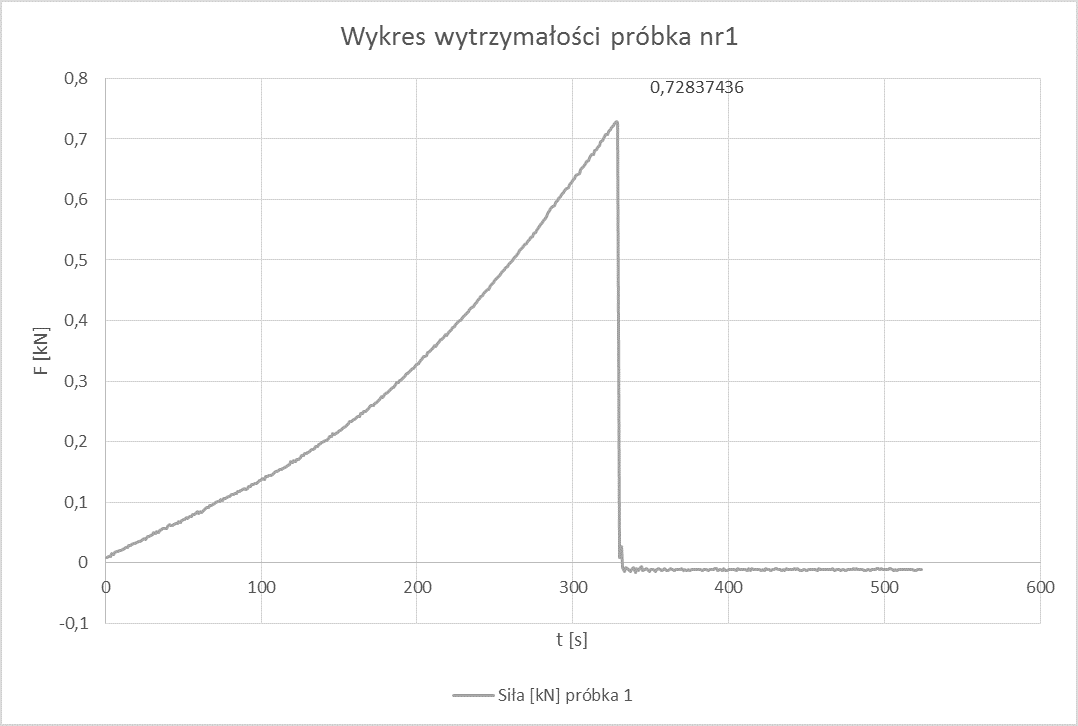
\includegraphics[width=1\textwidth]{sample1roz}
	\caption{Wykres przebiegu sił w trakcie próby na rozciąganie(próbka 1)}
\end{figure}

\begin{figure}
	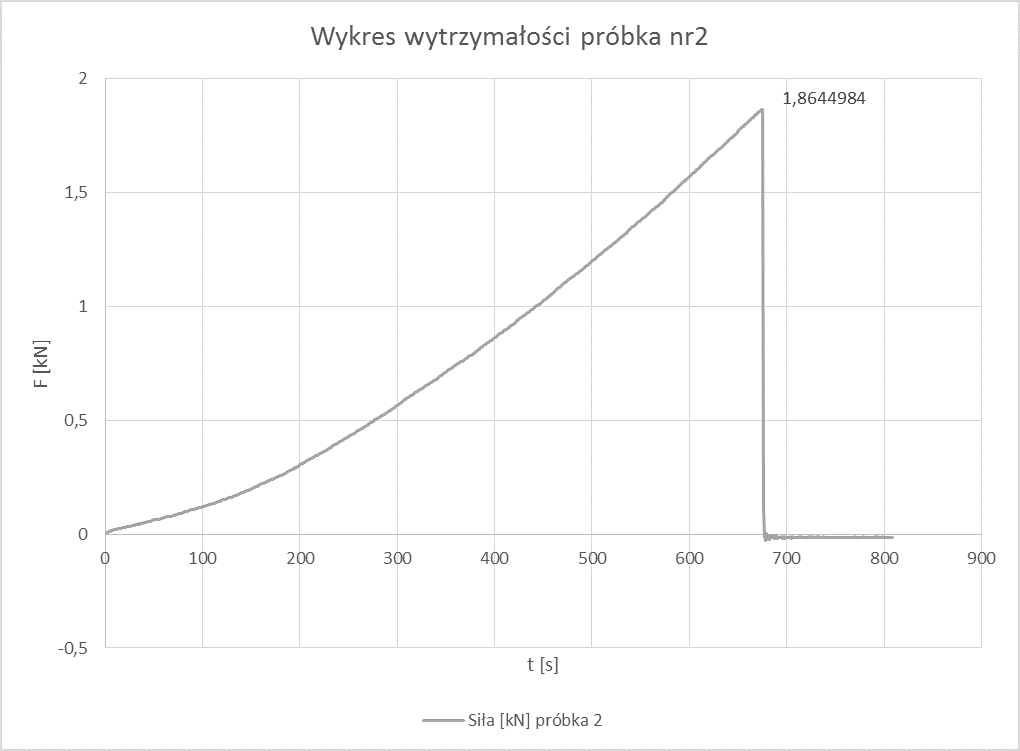
\includegraphics[width=1\textwidth]{sample2roz}
	\caption{Wykres przebiegu sił w trakcie próby na rozciąganie(próbka 2)}
\end{figure}

\begin{figure}
	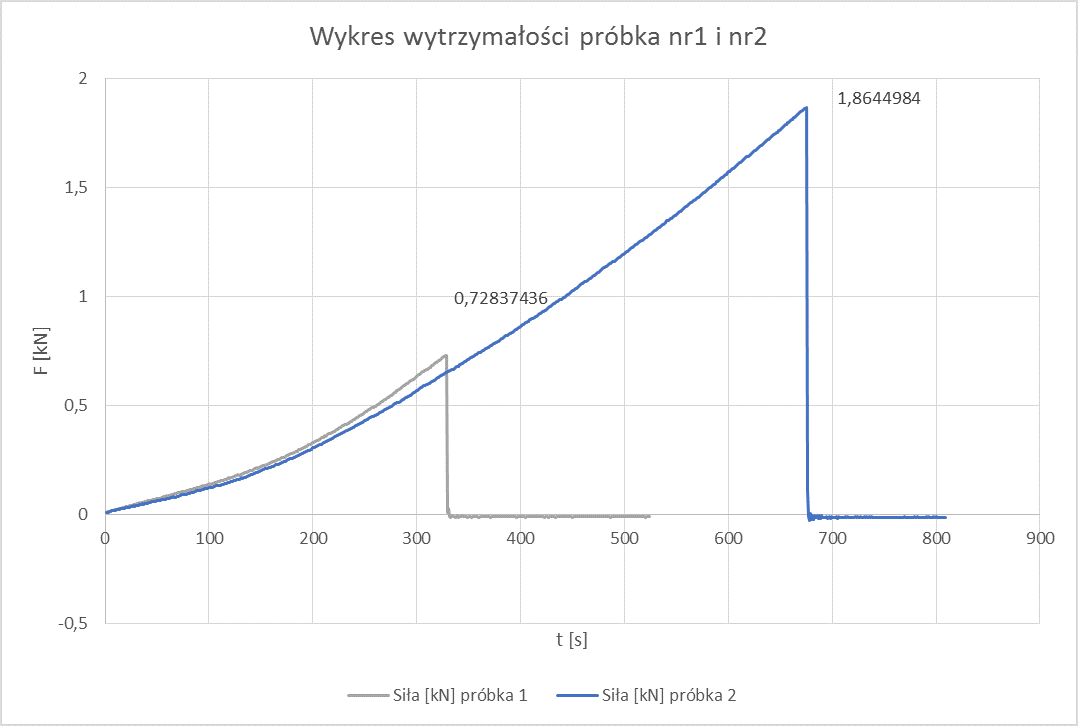
\includegraphics[width=1\textwidth]{bothsamplesroz}
	\caption{Wykres przebiegu sił w trakcie próby na rozciąganie}
\end{figure}

\subsection{Badania zgładów mikroskopowych}

\chapter{Opracowanie wyników badań}
\chapter{Podsumowanie i wnioski}

\nocite{*}
\bibliography{bibmag}
\bibliographystyle{plplain}

\end{document}